\chapter{Betrag, Kreis, Ungleichungen}

%\section{Kreise}
%\begin{enumerate}
%	\item Mittelpunkt: $ M \ = \ (0,0) $ ; Radius: $ r \ = \ 5 $
%		\[x^2 \ + \ y^2 \ = \ 25\]
%	\item Mittelpunkt: $ M \ = \ (5,0) $ ; Radius: $ r \ = \ 3 $
%		\[(x-5)^2 \ + \ y^2 \ = \ 9\]
%	\item Mittelpunkt: $ M \ = \ (-6.5,-8.5) $ ; Radius: $ r \ = \ 1.5 $
%		\[(x \ + \ 6.5)^2 \ + (y \ + \ 8.5)^2 \ = \ 2.25\]
%	\item Mittelpunkt: $ M \ = \ (6,0) $ ; Radius: $ r \ = \ 3 $ \\
%		Kreisgleichung w\"are: $ (x-6)^2 \ + \ y^2 \ = 9 $ \\
%		Umformung: $ y \ = \ \pm \ \sqrt{9 \ - \ (x \ - \ 6)^2} $ \\
%		Oberer Halbkreis: $ y \ = \ + \ \sqrt{9 \ - \ (x \ - \ 6)^2} $
%	\item Mittelpunkt: $ M \ = \ (-3,-3) $ ; Radius: $ r \ = \ 3 $ \\
%		Kreisgleichung w\"are: $ (x \ + \ 3)^2 \ + \ (y \ + \ 3)^2 \ = \ 9 $ \\
%		Unterer Halbkreis: $ y \ = \ - \sqrt{9 \ - \ (x \ + \ 3)^2} \ - \ 3 $		
%\end{enumerate}

\section{Betrag}
\begin{enumerate}
%\begin{multicols}{2}
\item $|x| = 7\\
	  x_1=7, x_2= -7$
\item $|x + 5| = 10$\newline
		1. Fall:\newline
		$(x+5) = 10 \rightarrow x=5$ \newline
		2.Fall:  \newline
		$-(x+5)=10 \rightarrow x=-15$

\item $|2x - 3| = 1$ \newline
	 	1. Fall:\newline
		$(2x-3) = 1 \rightarrow x=2$ \newline
		2.Fall:  \newline
		$-(2x-3)=1 \rightarrow x=1$
\item $|2x - 4| = 6x + 36$ \newline
		1. Fall:\newline
		$(2x-4) = 6x+36 \rightarrow x=-10$ \newline
		2.Fall:  \newline
		$-(2x-4)=6x+36 \rightarrow x=-4$
%\end{multicols}
\end{enumerate}

\section{Kreis}
\begin{enumerate}
\item \begin{enumerate}
		\item $M(1|3); P(4|3)$ \newline
		allgemeine Kreisgleichung: $(x-x_m)^2 + (y-y_m)^2 =r^2$ \newline
		einsetzen: $(4-1)^2 + (3-3)^2 =r^2\\
		\rightarrow r=3\\
		\curvearrowright (x-1)^2+(y-3)^2 = 3$
		
		\item $M(-1|5); P(6|-4)$ \newline
		einsetzen: $(6+1)^2 + (-4-5)^2 =r^2\\
		\rightarrow r=\sqrt{130}\\
		\curvearrowright (x+1)^2+(y-5)^2 = \sqrt{130}$
		
		\item $M(-2|-1); P(4|3)$ \newline
		einsetzen: $(4+2)^2 + (3+1)^2 =r^2\\
		\rightarrow r=\sqrt{52}\\
		\curvearrowright (x+2)^2+(y+1)^2 = \sqrt{52}$
		
		\end{enumerate}
		
	\item \begin{enumerate}
			\item $x^2 + y^2 - 4x - 2y + 5 = 4$ \newline
			nach binomischer Formel zu Kreisgleichung umstellen:\newline
			$ (x^2-4x)+ (y^2-2y) = -1 \\
			(x-2)^2 -4 + (y-1)^2 -1 = -1 \\
			(x-2)^2 + (y-1)^2 = 4$\newline \newline
			$\curvearrowright$ Kreis mit $M(2|1)$ und $r= 2$
			
			\item $ x^2 + y^2 +6x +2y+10 =1$ \newline
			nach binomischer Formel zu Kreisgleichung umstellen:\newline
			$ (x^2+ 6x) + (y^2 + 2y) = -9 \\
			(x+3)^2 -9 +(y+1)^2 -1 = -9\\
			(x+3)^2 +(y+1)^2 = 1\\ \\
			\curvearrowright$ Kreis mit $M(-3|-1)$ und $r=1$ 
			\end{enumerate}
			
		\item $P_1(6|7); P_2(2|9); P_3(-1|0)$ \newline \newline
		Aufstellen der Kreisgleichungen:\newline
		 $1. (6-x_m)^2 + (7-y_m)^2 = r^2\\
		 2.  (2-x_m)^2 + (9-y_m)^2 = r^2\\
		 3.  (-1-x_m)^2 + (-y_m)^2 = r^2$ \newline \newline
		Gleichsetzen von 1 und 2; 2 und 3: \newline
		$(6-x_m)^2 + (7-y_m)^2 = (2-x_m)^2 + (9-y_m)^2$ \newline
		$(2-x_m)^2 + (9-y_m)^2 = (-1-x_m)^2 + (-y_m)^2$ \newline \newline
		Aufl\"osen und Zusammenfassen: \newline
		$4y_m= 8x_m\\
		84-6x_m = 18y_m$ \newline \newline
		Umstellen nach $x_m$ und Gleichsetzen: \newline
		$\dfrac{1}{2}y_m = 14- 3y_m\\
		\curvearrowright y_m = 4$ \newline \newline
		Einsetzen des Ergebnisses: \newline
		$ x_m = \dfrac{1}{2}y_m = \dfrac{1}{2}* 4 = 2\\
		r=\sqrt{(6-2)^2 + (7-4)^2} = \sqrt{25} = 5$ \newline \newline
		$\curvearrowright$ Kreis: $(x-2)^2 + (y-4)^2 = 5$
		


\end{enumerate}
\section{Ungleichungen}

\subsection{Ungleichungen mit einer Variablen}

\begin{enumerate}
	\item Aufgabe:
					\[f : (x \ + \ 1)(x \ - \ 1) \ \leq 0\]
					\[g : \sqrt x \geq 1 \]
				L\"osung:
					\[-1 \ \leq \ x \ \leq \ 1\]
					\begin{center}
						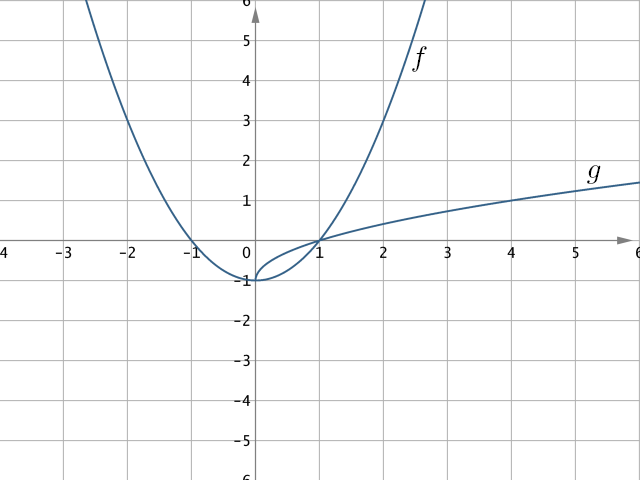
\includegraphics[width=0.5\textwidth]{img/Aufgaben/Analytisch/A1.PNG}
					\end{center}
	\item Aufgabe:
					\[f : \sqrt{\frac 1 2 x^3 \ + \ 2x^2 \ + \ \frac {21} 8 x \ + \ \frac 9 8} \ < \ \sqrt{\frac 1 2 x^2 \ + \ \frac 3 2 x \ + \ \frac 9 8 } \]
				Zwischenschritte: 
	  			\[ \sqrt{ (\frac 1 {\sqrt 2} x \ + \ \frac 3 {\sqrt 2})^2 ( x \ + \ 1)} \ < \ \frac 3 2 \sqrt{(\frac 1	{\sqrt 2} x \ + \ \frac 3 {\sqrt 2})^2}\]
	  			\[\sqrt {(x \ + \ 1)} \ < \ \frac 3 2\]
	  		L\"osung:
	  			\[0 \ < x \ < \ \frac 5 4\]
	  			\begin{center}
						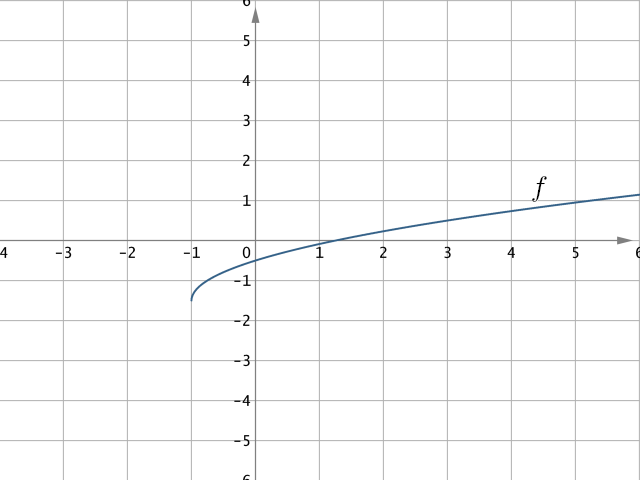
\includegraphics[width=0.5\textwidth]{img/Aufgaben/Analytisch/A2.PNG}
					\end{center}
	\item Aufgabe:
					\[f : \frac 1 2 x^2 \ - \ 1 \ > \ 0\]
				L\"osung:
					\[x \ < \ \sqrt 2 \ \cup \ x \ > \ \sqrt 2\]
					\begin{center}
						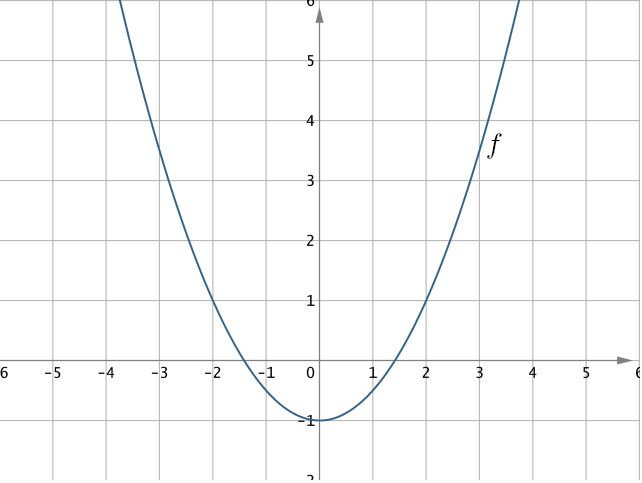
\includegraphics[width=0.5\textwidth]{img/Aufgaben/Analytisch/A3.PNG}
					\end{center}
	\item Aufgabe:
					\[f : x^3 \ + \ 3x^2 \ - \ 4 \ > \ 0\]
				Zwischenschritt:
					\[(x \ - \ 1)(x \ + \ 2)^2 \ > \ 0\]
				L\"osung:	
					\[1 \ < \ x\]
					\begin{center}
						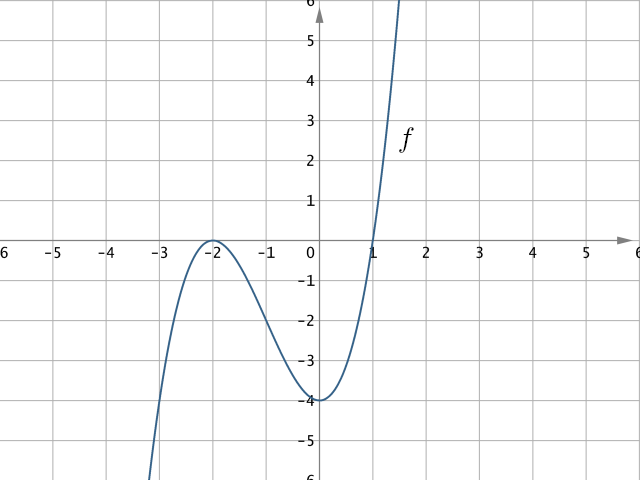
\includegraphics[width=0.5\textwidth]{img/Aufgaben/Analytisch/A4.PNG}
					\end{center}
	\item Aufgabe:
					\[f : x^3 \ + \ 3x^2 \ + \ 3x \ + \ 1 < 0\]
				Tipp: Pascallsches Dreieck \\
				Zwischenschritt:
					\[(x \ + \ 1)^3 < 0\]
				L\"osung:
					\[x \ < \ -1\]
					\begin{center}
						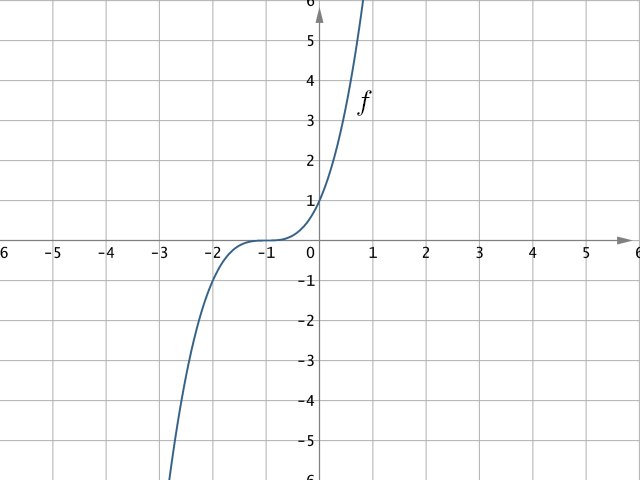
\includegraphics[width=0.5\textwidth]{img/Aufgaben/Analytisch/A5.PNG}
					\end{center}
	\item Aufgabe:
					\[f : x^6 \ - \ 6x^5 \ + \ 15x^4 \ - \ 20x^3 \ + \ 15x^2 \ - \ 6x \ + \ 1 \ \leq \ 0\]
				Nochmal: Pascallsches Dreieck \\
				Zwischenschritt:
					\[(x \ - \ 1)^6 \ \leq \ 0\]
				L\"osung:
					\[x \ \geq \ 1\]
					\begin{center}
						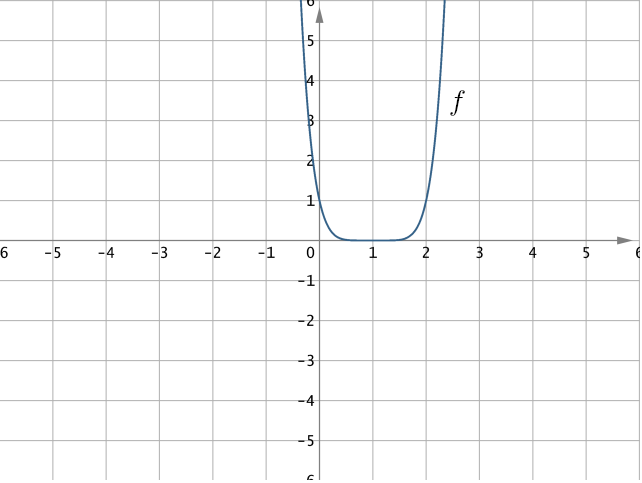
\includegraphics[width=0.5\textwidth]{img/Aufgaben/Analytisch/A6.PNG}
					\end{center}
	\item Aufgabe:
					\[f : \frac 1 2 x^2 \ - \ 8 \ > \ 0\]
					\[g : -3(x \ - \ 1)^2 \ + \ 12 \ > \ 0\]
				L\"osung: \\
					1.Gl: $ x^2 \ > \ 16 \rightarrow x \ > \ 4 \ \cup \ x \ < \ -4 $ \\
					2.Gl: $ -1 \ < \ x \ < \ 3 $ \\
	 				keine L\"osung!
	 				\begin{center}
						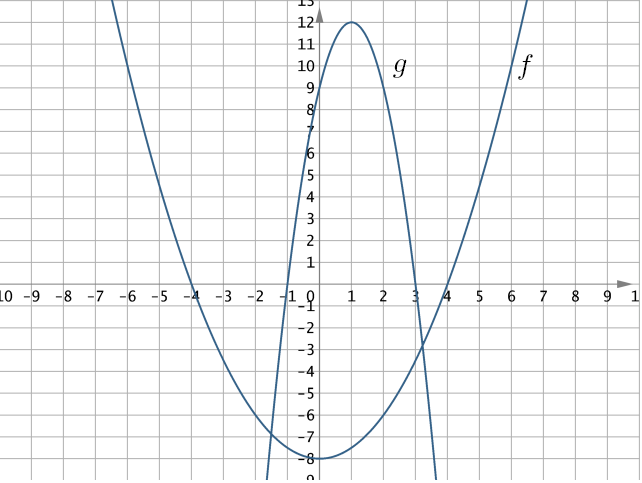
\includegraphics[width=0.5\textwidth]{img/Aufgaben/Analytisch/A7.PNG}
					\end{center}
	\item Aufgabe:
					\[f : (x^2 \ - \ 2)(x \ + \ 1) \ \geq \ 0\]
				L\"osung:
					\[ - \sqrt 2 \ < \ x \ < \ -1 \ \cup \ x \ > \ \sqrt 2\]
					\begin{center}
						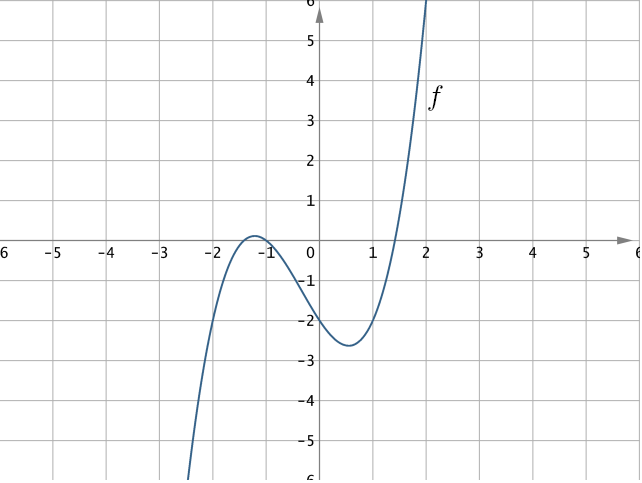
\includegraphics[width=0.5\textwidth]{img/Aufgaben/Analytisch/A8.PNG}
					\end{center}
	\item Aufgabe:
					\[f : ax^2 \ > \ 0\]
					\[g : \frac 1 2 x \ + \ 1 > 0\]
				L\"osung: \\
					1.Gl: $ x \in \mathbb{R} \setminus \lbrace 0 \rbrace $ \\
					2.Gl: $ x \ > \ -2 $
					\[x \ > \ -2 \ und \ x \ \neq \ 0\]
					\begin{center}
						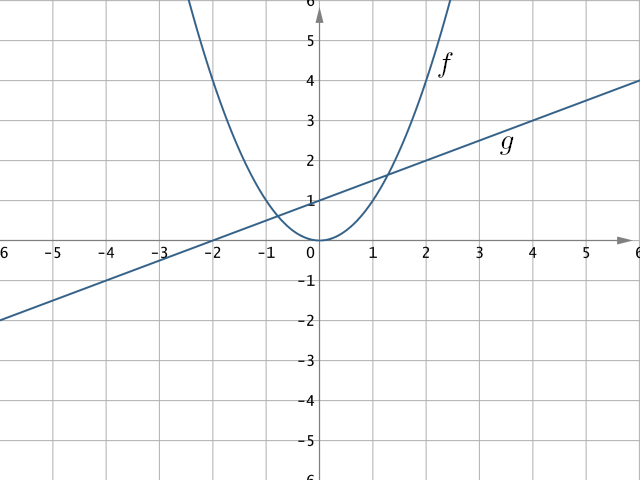
\includegraphics[width=0.5\textwidth]{img/Aufgaben/Analytisch/A9.PNG}
					\end{center}
	\item Aufgabe:
					\[f : x^2 \ + \ a \ > \ 0\]
					\[g : \frac 1 2 x \ + \ 1 \ > \ 0\]
				L\"osung: \\
					1.Gl: \\
						\begin{tabular}{|l|l|}
							\hline $ x \in \mathbb{R} $ & $ a \ > \ 0 $ \\
							\hline $ x \in \mathbb{R} \setminus \lbrace 0 \rbrace $ & $ a \ = \ 0 $ \\
							\hline $ x \ < \ -\sqrt a \ \cup \ x \ > \ \sqrt a \ \  $ & $ a \ < \ 0 $ \\
							\hline
						\end{tabular} \\
					2.Gl: $ x \ > \ -2 $ \\
					\begin{center}
					\begin{tabular}{|l|l|}
						\hline $ x \ > \ -2 $ & $ a \ > \ 0 $ \\
						\hline $ x \ > \ -2 \ $ und $ \ x \ \neq \ 0 $ & $ a \ = \ 0 $ \\
						\hline $ -2 \ < \ x \ < \ -\sqrt a \ \cup \ x \ > \ \sqrt a $ & $ -4 \ < \ a \ < \ 0 $ \\
						\hline $ x \ > \ \sqrt a $ & $ a \ \leq \ -4 $ \\
						\hline
					\end{tabular}
					\end{center}
					\begin{center}
						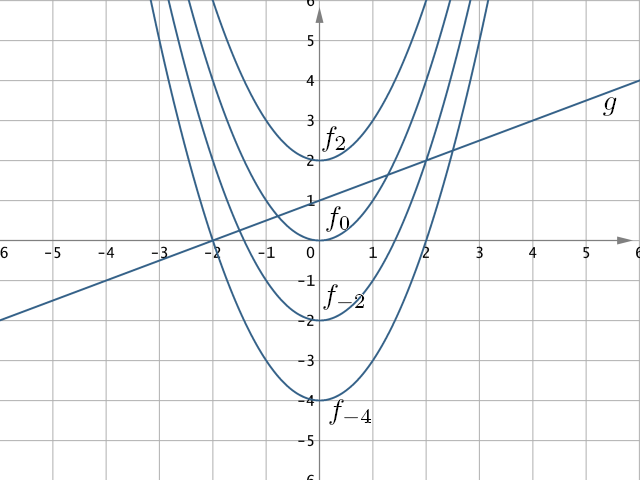
\includegraphics[width=0.5\textwidth]{img/Aufgaben/Analytisch/A10.PNG}
					\end{center}
	\item Aufgabe:
					\[f : -x^2 \ + \ a \ < \ 0\]
					\[g : x \ + \ a \ < \ 0\]
				L\"osung: \\
					1.Gl: \\
						\begin{tabular}{|l|l|}
							\hline $ x \ < \ -\sqrt a \ \cup \ x \ > \sqrt a $ & $ a \ > \ 0 $ \\
							\hline $ x \in \mathbb{R} \setminus \lbrace 0 \rbrace $ & $ a \ = \ 0 $ \\
							\hline $ x \in \mathbb{R} $ & $ a \ < \ 0 $ \\
							\hline
						\end{tabular} \\
					2.Gl: $ x \ < \ -a $
					\begin{center}
					\begin{tabular}{|l|l|}
						\hline $ x \ < \ -a $ & $ a \ > 1 $ \\
						\hline $ x \ < \ -\sqrt a $ & $ 0 \ < \ a \ <= \ 1 $ \\
						\hline $ x \ < \ 0 $ & $ a \ = \ 0 $ \\
						\hline $ x \ < \ -a $ & $ a \ < \ 0 $ \\
						\hline
					\end{tabular}
					\end{center}
					\begin{center}
						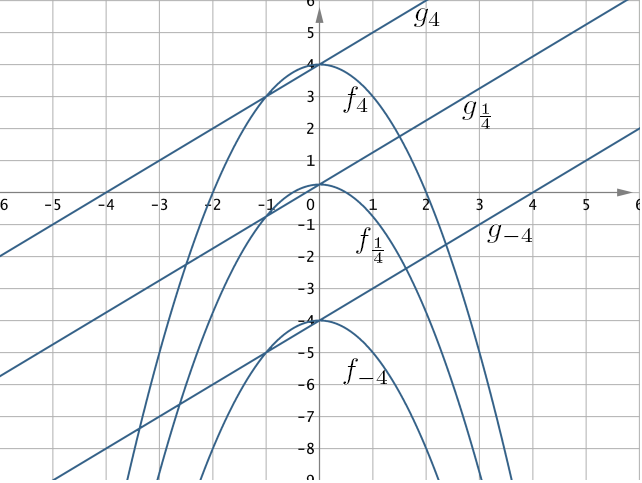
\includegraphics[width=0.5\textwidth]{img/Aufgaben/Analytisch/A11.PNG}
					\end{center}
	\item Aufgabe: 
					\[f : 4x^2 \ - \ 2ax \ + \ \frac 1 4 a^2 \ \geq \ 0\]
				Zwischenschritt:
					\[(x \ - \ \frac 1 4 a)^2 \ \geq \ 0\]
				L\"osung:
					\[x \in \mathbb{R} \setminus \lbrace \frac 1 4 a \rbrace\]
					\begin{center}
						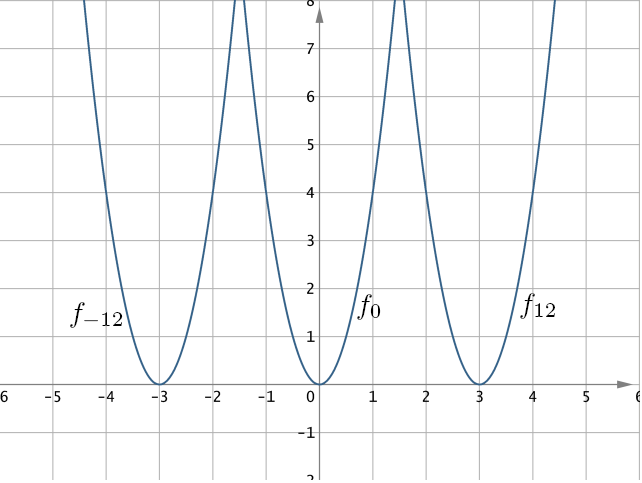
\includegraphics[width=0.5\textwidth]{img/Aufgaben/Analytisch/A12.PNG}
					\end{center}
	\item Aufgabe:
					\[f : x^3 \ + \ x^2 \ - \ 2x \ \geq \ 2\]
					(siehe Aufgabe 8) \\
				L\"osung:
					\[ - \sqrt 2 \ < \ x \ < \ -1 \ \cup \ x \ > \ \sqrt 2\]
					\begin{center}
						\includegraphics[width=0.5\textwidth]{img/Aufgaben/Analytisch/A13.PNG}
					\end{center}
	\item Aufgabe:
					\[f : (x \ - \ 1)^2 \ - \ 4 \ < \ 0\]
					\[g : -(x \ + \ 1)^2 \ + \ 4 \ > \ 0\]
				L\"osung: \\
					1.Gl: $ -1 \ < \ x \ < \ 3 $ \\
					2.Gl: $ -3 \ < \ x \ < \ 1 $ \\
					\[-1 \ < \ x \ < \ 1\]
					\begin{center}
						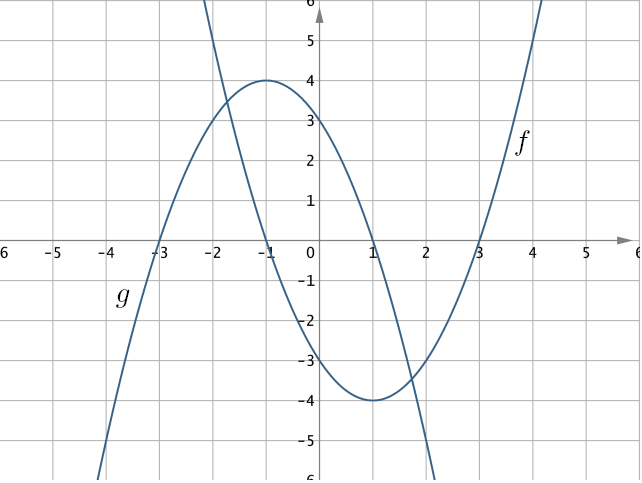
\includegraphics[width=0.5\textwidth]{img/Aufgaben/Analytisch/A14.PNG}
					\end{center}
	\item Aufgabe:
					\[f : \sqrt {(x-1)} \ \geq \ 0\]
					\[g : - \frac 1 4 x \ + \ 4 \ < \ 0\]
				L\"osung: \\
					1.Gl: $ x \ \geq \ 1 $ \\
					2.Gl: $ x \ > \ 16 $
					\[ x \ > \ 16\]
					\begin{center}
						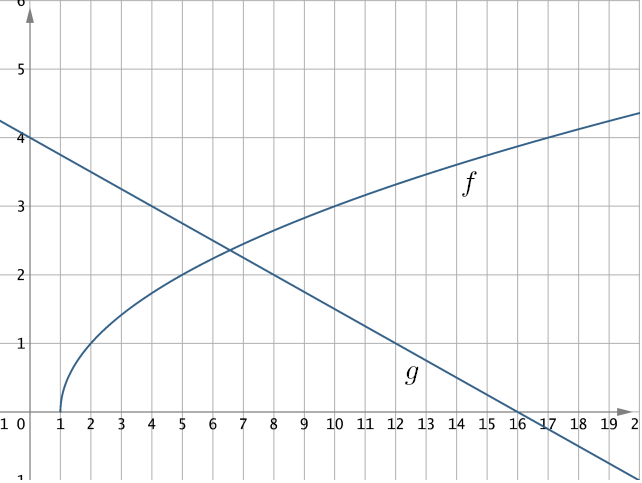
\includegraphics[width=0.5\textwidth]{img/Aufgaben/Analytisch/A15.PNG}
					\end{center}
	\item Aufgabe:
					\[f : x^4 \ - \ 16 \ \leq \ 0\]
					\[g : x^3 \ + \ 1 \ \geq \ 0\]
				L\"osung: \\
					1.Gl: $ -2 \ \leq \ x \ \leq \ 2 $ \\
					2.Gl: $ x  \ \geq \ -1 $ \\
					\[-1 \ \leq \ x \ \leq \ 2\]
					\begin{center}
						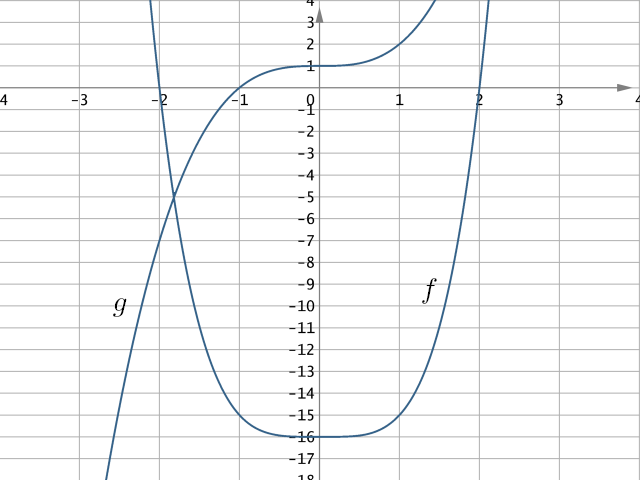
\includegraphics[width=0.5\textwidth]{img/Aufgaben/Analytisch/A16.PNG}
					\end{center}
\end{enumerate}

\subsection{Ungleichungen mit mehreren Variablen}

\begin{enumerate}
	\item Aufgabe: 
					\[f : x^2 \ + \ y^2 \ < \ 25 \]
					\[g : \frac 1 2 x \ + \ \frac 5 2 \ > \ y \]
					\[h : -x \ - \ 5 \ < \ y \]
				L\"osung:
				\begin{center}
						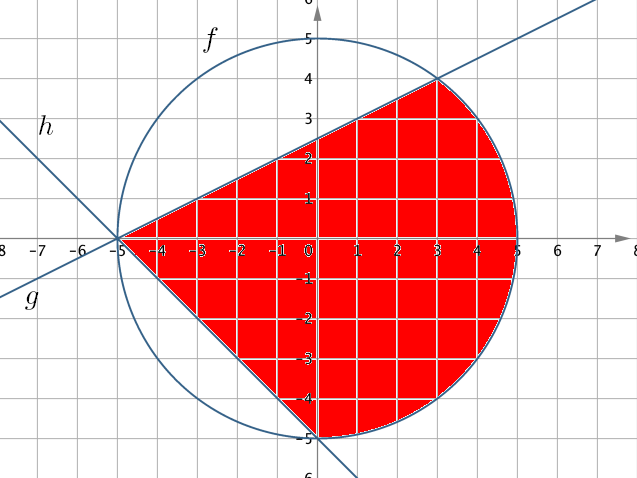
\includegraphics[width=0.5\textwidth]{img/Aufgaben/Graphisch/A1.PNG}
				\end{center}
	\item Aufgabe:
					\[f : - x^2 \ + \ 5 \ < \ y \]
					\[g : x(x \ - \ 3)^2 \ > \ y \]
					\[h : -x \ - \ 2 \ > \ y \]
				L\"osung:
					\begin{center}
						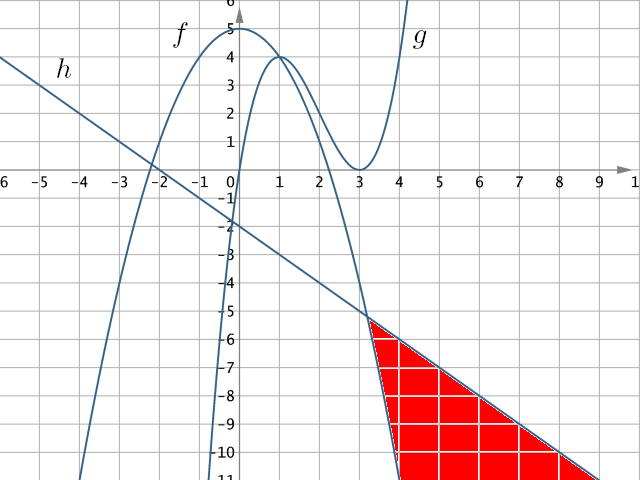
\includegraphics[width=0.5\textwidth]{img/Aufgaben/Graphisch/A2.PNG}
					\end{center}
	\item Aufgabe:
					\[f : 3x^2 \ - \ 3x \ - \ 10 \ < \ -4 \ + \ y \]
					\[g : y \ \leq \ \frac 1 2 \]
				L\"osung:
					\begin{center}
						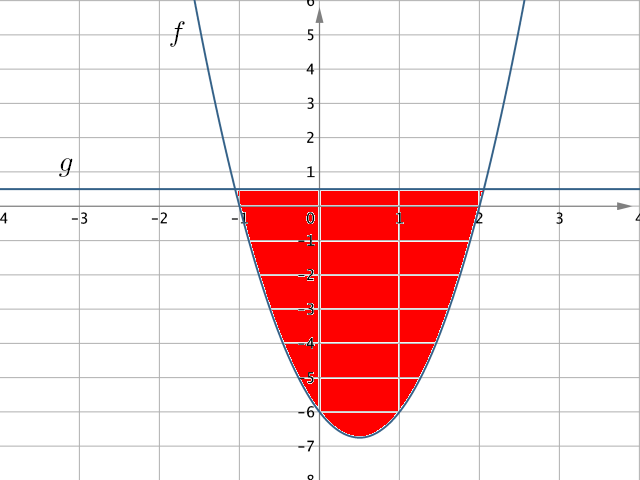
\includegraphics[width=0.5\textwidth]{img/Aufgaben/Graphisch/A3.PNG}
					\end{center}
	\item Aufgabe:
					\[f : y \ < \ \frac {2x^2 \ + \ 3x \ + \ 4} {- x^4 \ - \ 2x^3 \ - \ x^2 \ + \ 4x \ + \ (2x \ + \ x^2)^2} \]
					\[g : - \frac 1 x \ < \ y \]
					\[h : - ( \frac 1 {\sqrt 2} x )^2 \ < \ y \ - \ \frac 1 2 x^2 \ + \ \frac 1 2 x \ + \ 2 \]
					\[i : y \ + \ x \ - \ 2 \ < \ 0 \]
				Zwischenschritt:
				\[f : y \ < \ \frac 1 x\]
				\[h : y \ > \ -\frac 1 2 x \ - \ 2\]
				L\"osung:
					\begin{center}
						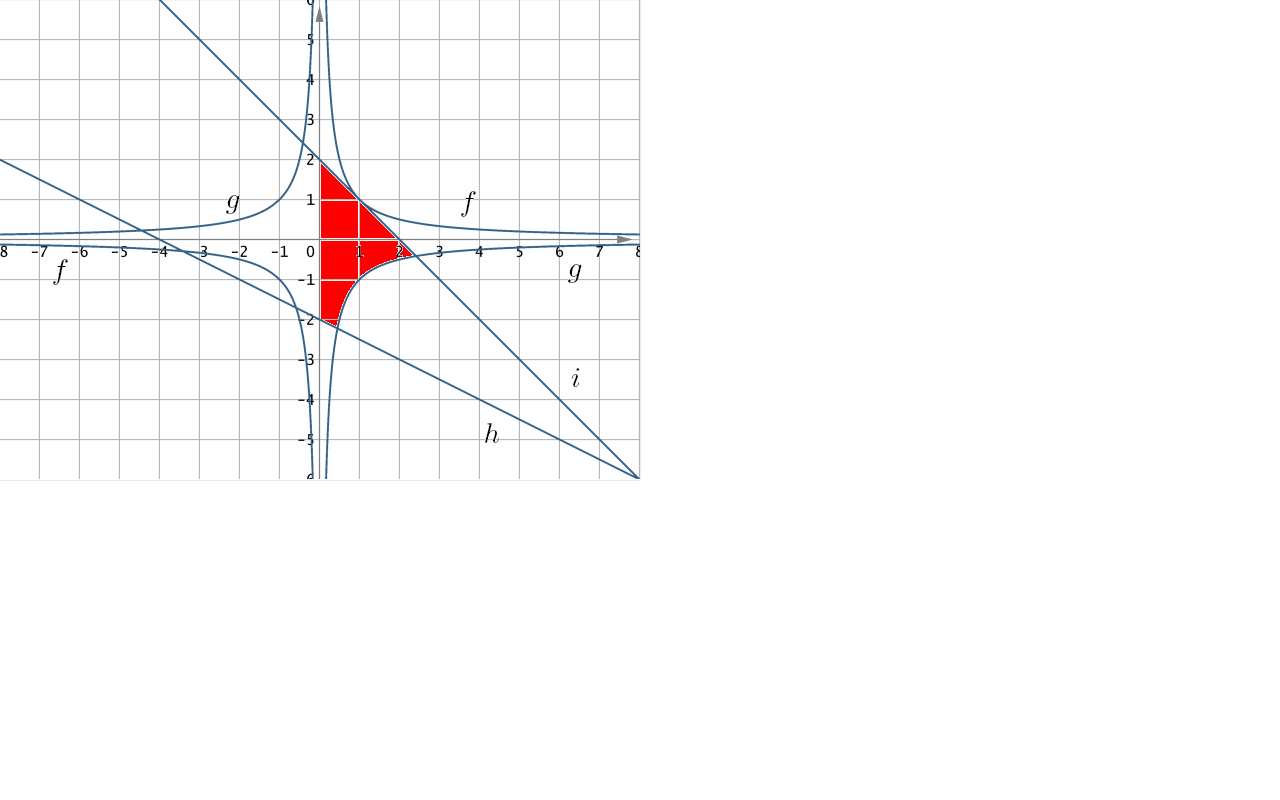
\includegraphics[width=0.5\textwidth]{img/Aufgaben/Graphisch/A4.PNG}
					\end{center}
	\item Aufgabe:
					\[f : \frac 1 2 x^2 \ - \ 3x \ \leq \ y\]
					%\[g : \frac 4x^3 \ + \ 2x^2 \ - \ \frac {13} 4 x \ \geq \ y\]
					\[g : y \ \leq \ -x\]
					\[h : 17x^3 \ - \ \frac 1 2 \ = \ y\]
				L\"osung:
					\begin{center}
						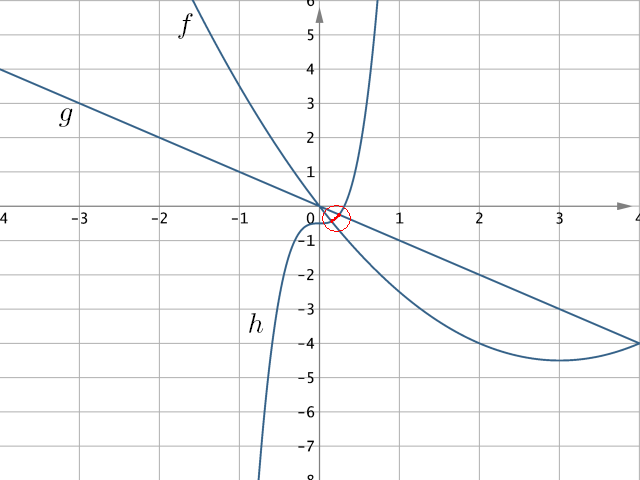
\includegraphics[width=0.5\textwidth]{img/Aufgaben/Graphisch/A5.PNG}
					\end{center}
	\item Aufgabe:
					\[f : y \ + \ \sqrt {\frac {x^3 \ + \ x^2 \ - \ x \ - \ 1} {x \ - \ 1}} \ > \ 0 \]
					\[g : \frac 2 {20} x \ - \ \frac 1 3 y \ + \ \frac 3 {12} \ < \ 0\]
				Zwischenschritt:
				\[f : y \ > \ -x \ - \ 1\]
				\[g : y \ > \ \frac {10} 3 x \ + \ \frac 3 4\]
				L\"osung:
					\begin{center}
						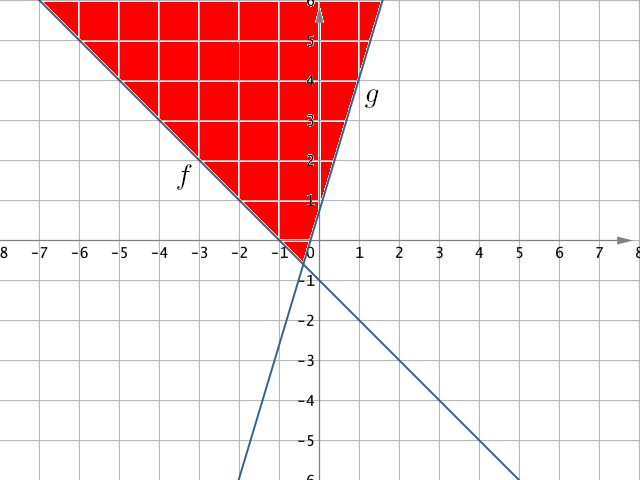
\includegraphics[width=0.5\textwidth]{img/Aufgaben/Graphisch/A6.PNG}
					\end{center}
	\item Aufgabe:
					\[f : \frac 1 2 x \ - \ 2 < y\]
					\[g : \frac 1 2 x \ + \ 2 > y\]
					\[h : 2 x \ - \ 4 < y\]
					\[i : 2 x \ + \ 4 > y\]
					\[k : - \frac 1 2 x \ - \ 2 < y\]
					\[l : - \frac 1 2 x \ + \ 2 > y\]
					\[m : -2 x \ - \ 4 < y\]
					\[n : -2 x \ + \ 4 > y\]
				L\"osung:
					\begin{center}
						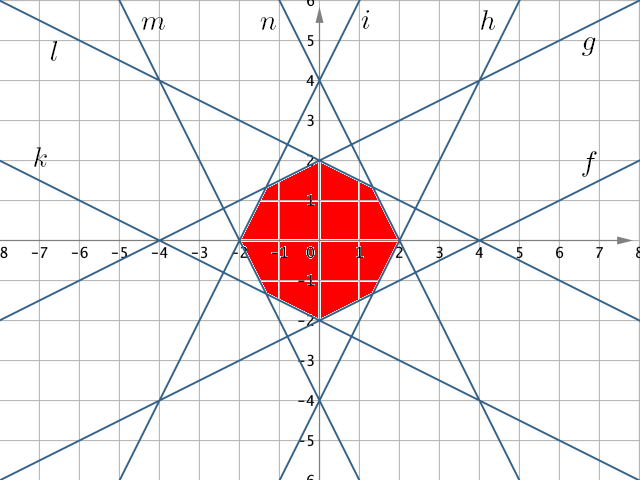
\includegraphics[width=0.5\textwidth]{img/Aufgaben/Graphisch/A7.PNG}
					\end{center}
	\item Aufgabe:
					\[f : |(x^2 \ + \ (y \ - \ 1)^2| \ = \ 4 \]
					\[g : x \ \geq \ y \]
				L\"osung:
					\begin{center}
						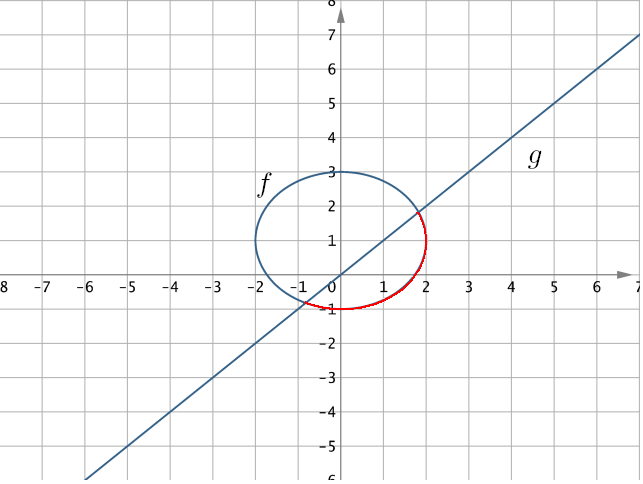
\includegraphics[width=0.5\textwidth]{img/Aufgaben/Graphisch/A8.PNG}
					\end{center}
	\item Aufgabe:
					\[f : ((\sin x) \ + \ \frac 1 2)^2 \ - \ \frac 3 4 \ - \ y \ - \ (\sin x)^2 < 0\]
					\[g : \cos (x \ + \ \frac {\pi} 2 ) + \ \frac 1 2 \ < \ y \]
				Zwischenschritt:
					\[f : y \ < \ \sin x \ - \ \frac 1 2\]
				L\"osung:
					\begin{center}
						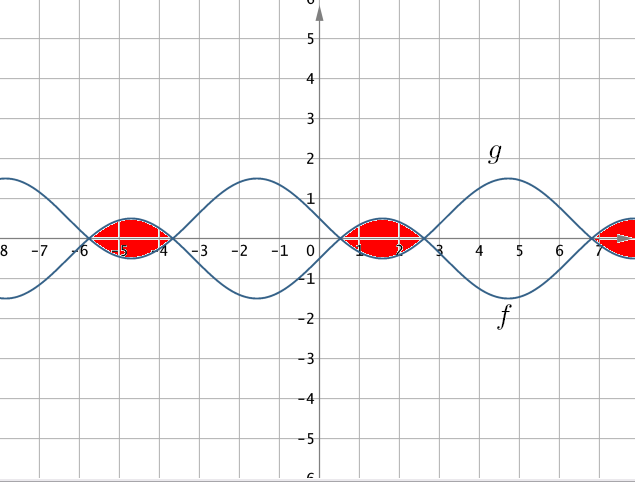
\includegraphics[width=0.5\textwidth]{img/Aufgaben/Graphisch/A9.PNG}
					\end{center}
	\item Aufgabe:
					\[f : |\frac 1 x| \ > y \]
					\[g : - \frac {1 \ + \ 7x^2} {x^2 y} > \ - \frac {y \ + \ 7} y\]
					\[h : |x| + y < 5\]
				Zwischenschritt:
					\[g : y \ > \ \frac 1 {x^2}\]
				L\"osung:
					\begin{center}
						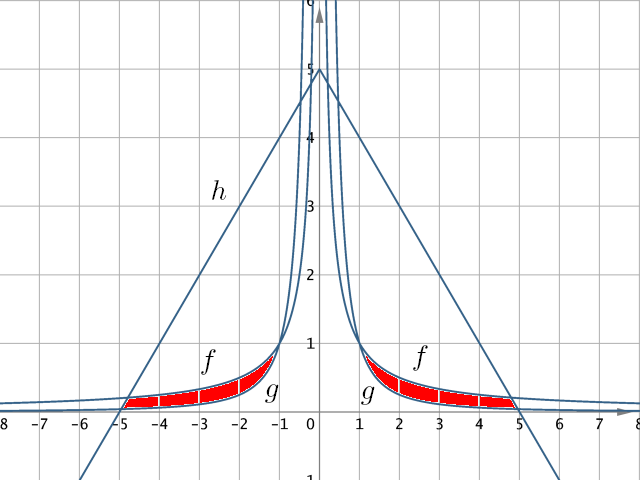
\includegraphics[width=0.5\textwidth]{img/Aufgaben/Graphisch/A10.PNG}
					\end{center}
	\item Aufgabe:
					\[f : 4x^2 \ + \ y^2 \ <= \ 16\]
					\[g : x^2 \ + \ 4y^2 \ <= \ 16\]
				L\"osung:
					\begin{center}
						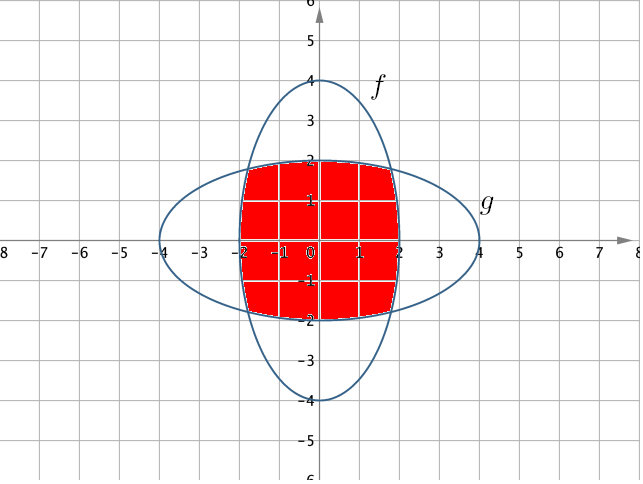
\includegraphics[width=0.5\textwidth]{img/Aufgaben/Graphisch/A11.PNG}
					\end{center}
	\item Aufgabe:
					\[f : (y \ - \ 2)^2 \ < \ 4 - (x \ - \ 2)^2\]
					\[g : y -2 < 0\]
					\[h : -|x \ - \ 2| \ + \ 2\ < \ y\]
				L\"osung:
					\begin{center}
						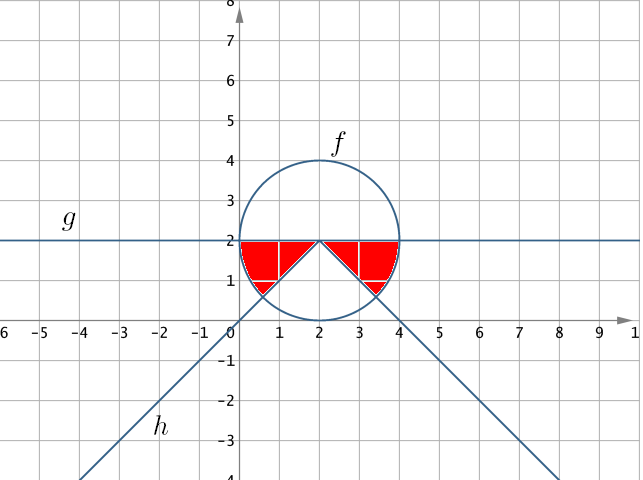
\includegraphics[width=0.5\textwidth]{img/Aufgaben/Graphisch/A12.PNG}
					\end{center}
	\item Berechnen Sie f\"ur die Ungleichung den Fl\"acheninhalt der L\"osungsmenge! \\
				Aufgabe:
					\[f : (2y \ - \ 3)^2 \ + \ (3y \ + \ 2)^2 \ + \ y \ - \ 10 \ \geq \ | \frac {4x \ + \ 4 (\frac 1 2 x \ - \frac 3 2 )^2 \ - \ 9} x | \ + \ 13y^2 \]
					\[g : y \ \leq \ -1\]
				Zwischenschritt:
					\[f : y \ \geq \ |x-2|-3\]
				L\"osung: Fl\"acheninhalt $ = \ 4 $
					\begin{center}
						\includegraphics[width=0.5\textwidth]{img/Aufgaben/Fl\"acheninhalt/A13.PNG}
					\end{center}
	\item Berechnen Sie f\"ur das Ungleichungssystem den Fl\"acheninhalt der L\"osungsmenge! \\
				Aufgabe:
					\[f : x^2 \ - \ 4x \ + 4 \ + \ y^2 \ - \ 2y \ + \ 1 \ \geq \ 1 \]
					\[g : (x \ - \ 2)^2 \ + \ (y \ - \ 2)^2 \ \leq \ 4 \]
					\[h : (x \ - \ 2)^2 \ + \ (y \ - \ 3)^2 \ \geq \ 1 \]
				Zwischenschritt:
					\[f : (x \ - \ 2)^2 + (y \ - \ 1)^2 \ \geq \ 1\]
				L\"osung: Fl\"acheninhalt $ = 4 \pi \ - \ 2 \pi \ = 2 \pi $
					\begin{center}
						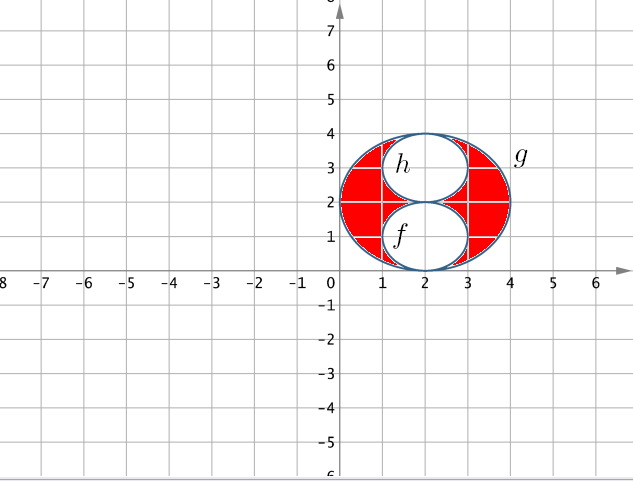
\includegraphics[width=0.5\textwidth]{img/Aufgaben/Fl\"acheninhalt/A14.PNG}
					\end{center}
	\item F\"ur welches a ist der Fl\"acheninhalt der L\"osungsmenge $ = 2 $ ?
				Aufgabe:
					\[f : y \ \geq \ 2\]
					\[g : -|x| \ + \ a \ \leq \ y\]
				L\"osung: Fl\"acheninhalt $ = 2 $ f\"ur $ a = 2 $
					\begin{center}
						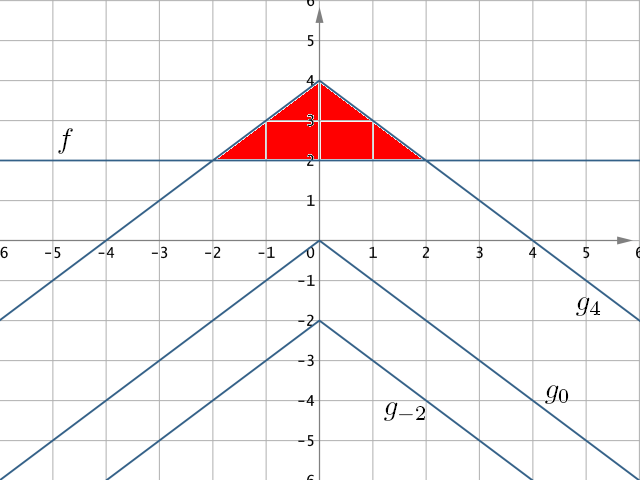
\includegraphics[width=0.5\textwidth]{img/Aufgaben/Fl\"acheninhalt/A15.PNG}
					\end{center}
	\item Bestimmen Sie ein $a$ und ein $ b $, f\"ur das der Fl\"acheninhalt der L\"osungsmenge $ 2 \pi $ ergibt! \\
				Aufgabe:
					\[f : - \frac 1 3 x \ \leq y \ - \ 2\]
					\[g : (x+ \frac 1 4 b)^2 \ + \ (y \ - \ \frac 3 2 a)^2 \ \leq \ a^2\]
				(einfachste) L\"osung: $ a = 2 $ , $ b = 12 $
					\begin{center}
						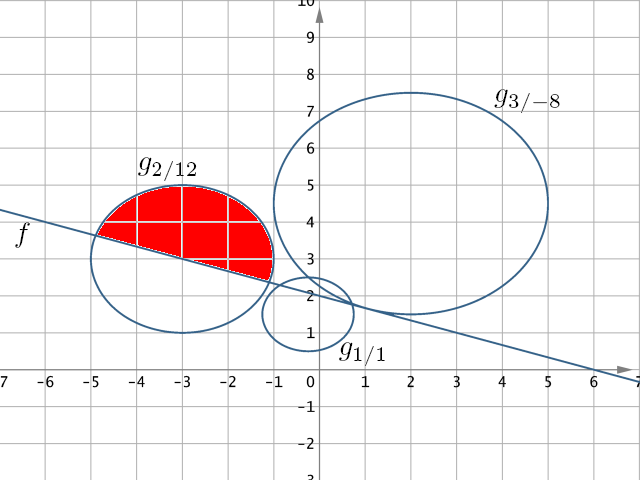
\includegraphics[width=0.5\textwidth]{img/Aufgaben/Fl\"acheninhalt/A16.PNG}
					\end{center}
	\item Beschreiben sie die L\"osungsmenge des Ungleichungssystems! \\
				Aufgabe:
					\[f : x^2 \ + \ y^2 \ + \ z (z \ + \ 2) \ < \ 8 \]
					\[g : x \ \leq \ 0 \]
					\[h : y \ \leq \ 0 \]
				Zwischenschritt:
					\[f : x^2 \ + \ y^2 \ + \ (z \ + \ 1)^2 \ < \ 9\]
				L\"osung: \\
				Die L\"osungsmenge ist eine Halbkugel unter der x-y-Ebene im $ \mathbb{R}^3 $, die um eine Einheit in z-Richtung verschoben ist.
	\item Beschreiben sie die L\"osungsmenge des Ungleichungssystems! \\
				Aufgabe:
					\[f : (x \ - \ 2 \sqrt 3)^2 \ + \ (x \ - \ 2 \sqrt 3)^2 \ + \ (z \ - \ 2 \sqrt 3)^2 \ \leq \ 36\]
					\[g : (x \ + \ 2 \sqrt 3)^2 \ + \ (x \ + \ 2 \sqrt 3)^2 \ + \ (z \ + \ 2 \sqrt 3)^2 \ \leq \ 36\]
				L\"osung: \\
				Es ist schnell ersichtlich, dass es sich mit zwei Kugeln mit Radius $ r = 6 $ handelt. 
				Bei n\"aherer Betrachtung ist zu erkennen, dass der Abstand des Mittelpunktes ebenfalls 6 betr\"agt.
				Da sich die Kugeln genau gegen\"uberliegen, haben sie nur den Ursprung als gemeinsame L\"osung.
				Die L\"osungsmenge ist somit nur der Punkt mit $ x = 0, y = 0, z = 0 $.
\end{enumerate}
